\subsection{Lentes y formación de imágenes}

Para empezar comencemos recordando que cuando un rayo de luz pasa de un medio con índice de refracción \(n_1\) a otro con índice \(n_2\), y atraviesa una superficie plana, la dirección del rayo cambia de acuerdo con la Ley de Snell:

\[
n_1 \sin \theta_1 = n_2 \sin \theta_2
\]

\subsubsection{Refacción en una superficie esférica}

Consideremos una única superficie esférica de radio \(R\), separando dos medios de índices \(n_1\) y \(n_2\). Un objeto colocado en el medio \(n_1\) yace frente a la superficie esférica en el punto \(O\). Los rayos que salen de \(O\) divergen y reflejan en la superficie esférica, formando un haz que converge en el punto \(I\). 

En la figura \ref{fig:lens_refraction} se muestra esta situación, pero solo se ha dibujado un rayo incidente y un rayo refractado para ilustrar la idea.
\begin{figure}[ht]
  \centering
  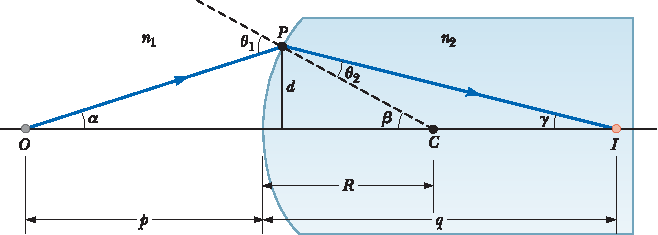
\includegraphics[width=\textwidth]{lens_refraction.pdf}
  \caption{Imagen formada por refracción en una superficie esférica.}
  \label{fig:lens_refraction}
\end{figure}

Para aproximaciones paraxiales\footnote{La aproximación paraxial se utiliza para el cálculo de sistemas ópticos, suponiendo que las trayectorias de los rayos de luz forman ángulos pequeños con el eje óptico.} (ángulos pequeños en radianes), se puede hacer \(\sin \theta \approx \tan \theta \approx \theta\), y se puede reescribir la ecuación de Snell como:
\[
  n_1 \theta_1 = n_2 \theta_2
\]

Se sabe que el ángulo externo de un triángulo es igual a la suma de los ángulos internos no adyacentes (ver demostración en la sección adicional: \ref{sec:suma_angulos_internos}). Así que:
\begin{align*}
  \theta_1 =& \alpha + \beta \\
  \beta =& \theta_2 + \gamma
\end{align*}
Si combina las tres expresiones y elimina \(\theta_1\) y \(\theta_2\), obtiene:
\begin{equation}
  n_1 \alpha + n_2 \gamma = (n_2 - n_1) \beta
\end{equation}

Y como estamos trabajando con aproximaciones paraxiales:
\begin{align*}
  \tan \alpha \approx &\alpha \approx \frac{d}{p} \\
  \tan \beta \approx &\beta \approx \frac{d}{R} \\
  \tan \gamma \approx &\gamma \approx \frac{d}{q}
\end{align*}
Podemos reescribir la expresión como sigue:
\begin{equation}
\frac{n_1}{p} + \frac{n_2}{q} = \frac{n_2 - n_1}{R}
\label{eq:refraction_spherical}
\end{equation}

Donde:
\begin{itemize}
  \item \(p\): distancia desde el objeto hasta la superficie (en el medio 1),
  \item \(q\): distancia desde la imagen hasta la superficie (en el medio 2),
  \item \(R\): radio de curvatura de la superficie (positivo si el centro de curvatura está del lado del medio 2),
  \item \(n_1\): índice de refracción del medio de entrada,
  \item \(n_2\): índice de refracción del medio de salida.
\end{itemize}

\begin{tcolorbox}[myconclusion]
  \textbf{Cuidado}: En los espejos, la luz se refleja y las imágenes reales (cuando ocurren) se forman del mismo lado que el objeto.
  En cambio, en la refracción (como con lentes), los rayos de luz se desvían y convergen al otro lado del medio, por lo que la imagen se forma detrás de la superficie refractante, no del mismo lado del objeto.
\end{tcolorbox}

\noindent Esto implica que los signos serán al revés que en los espejos, quedando la siguiente regla convencional de signos:
\begin{enumerate}
  \item El lado de la superficie en el cual se originan los rayos luminosos se define como \textit{delante de la superficie}. El otro lado se llama \textit{detrás de la superficie}.
  \item Identifique la localización del objeto \(p\) teniendo en cuenta:
    \begin{itemize}
      \item el objeto está delante de la superficie: \textit{objeto real} (positivo)
      \item el objeto está detrás de la superficie: \textit{objeto virtual} (negativo)
    \end{itemize}
  \item  Localización de la imagen \(q\):
    \begin{itemize}
      \item la imagen está detrás de la superficie: \textit{imagen real} (positiva)
      \item la imagen está delante de la superficie: \textit{imagen virtual} (negativa)
    \end{itemize}
  \item Altura de la imagen \(h'\):
    \begin{itemize}
      \item la imagen no es invertida: \(h' > 0\) (positiva)
      \item la imagen es invertida: \(h' < 0\) (negativa)
    \end{itemize}
  \item Distancia focal \(f\) y radio \(R\):
    \begin{itemize}
      \item Es positiva cuando el centro de curvatura está del lado del medio 2
      \item Es negativa cuando el centro de curvatura está del lado del medio 1
    \end{itemize}
\end{enumerate}

\subsubsection{Refacción en una superficie plana}

Para una superficie plana, el eje óptico es perpendicular a la superficie. Tomando la ecuación \ref{eq:refraction_spherical} y suponiendo que el radio de curvatura es infinito, obtenemos la ecuación de refracción para una superficie plana:
\begin{align}
  \frac{n_1}{p} + \frac{n_2}{q} &= 0 \notag \\
  q &= -\frac{n_1}{n_2} p
  \label{eq:refraction_plane}
\end{align}
donde:
\begin{itemize}
  \item \(p\) es la distancia del objeto a la superficie (en el medio 1),
  \item \(q\) es la distancia de la imagen a la superficie (en el medio 2),
  \item \(n_1\) y \(n_2\) son los índices de refracción.
\end{itemize}

\begin{wrapfigure}{l}{0.3\textwidth}
  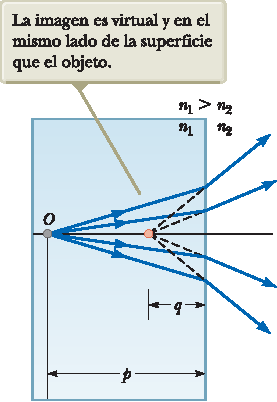
\includegraphics{plane_surface_refraction.pdf}
  \caption{Refacción en una superficie plana.}
  \label{fig:plane_surface_refraction}
\end{wrapfigure}
En el caso de la figura \ref{fig:plane_surface_refraction} se ha supuesto que \(n_1 > n_2\). Como cualquier índice de refracción es mayor que 1, para que se cumpla la ecuación \ref{eq:refraction_plane}, \(p\) y \(q\) deben tener signos opuestos, veamos si es así. En el caso de \(p\) sabemos que sería positivo, ya que está en el medio de índice \(n_1\), y según la ``regla de signos'' que establecimos es positivo. Por lo tanto, \(q\) debería ser negativo. Veamos: los rayos que salen de \(p\) se sabe que divergen, y como \(n_1 > n_2\), los rayos después del cruzar de medio también divergen entre sí, como se muestra en la figura \ref{fig:plane_surface_refraction}, esto implica que la imagen \(q\) estará del mismo lado que el objeto, formando una imagen virtual. Según nuestra regla de signos, \(q\) será negativo, lo que verifica la ecuación.

El caso ejemplificado suele ser el más común, donde por ejemplo se observa un pez bajo el agua. En ese caso, se supone que los rayos salen del pez, y como \(n_{\text{agua}} < n_{\text{aire}}\), el caso será similar a la figura \ref{fig:plane_surface_refraction}, donde la imagen será virtual. 

Sin embargo, si en algún caso \(n_1 < n_2\), los rayos también divergen, pero lo hacen más lentamente, y la imagen estará detrás del objeto.

\subsection{Imágenes formadas por lentes delgadas}

Una lente delgada es una combinación de dos superficies esféricas, muy cercanas entre sí comparadas con las distancias del objeto y la imagen. En este caso vamos a considerar una lente de espesor \(e \to 0\), es decir, una lente delgada como se muestra en la figura \ref{fig:lens_deduction}.
\begin{figure}[ht]
  \centering
  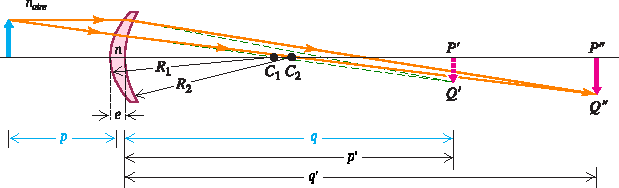
\includegraphics[width=\textwidth]{lens_deduction.pdf}
  \caption{Elementos y distancias de una lente delgada.}
  \label{fig:lens_deduction}
\end{figure}

La imagen formada por la primera superficie de una lente sirve como el objeto de la segunda superficie. Como la lente es delgada \(-q=p'\) por no estar en el lado entrante. 

Necesitamos aplicar la ecuación de una sola superficie a cada superficie \(s_1\) y \(s_2\).

\subparagraph{Para \(s_1\):}

\begin{equation*}
  \frac{n_\text{aire}}{p} + \frac{n}{q} = \frac{n - n_\text{aire}}{R_1}
\end{equation*}

\subparagraph{Para \(s_2\):}

\begin{equation*}
  \frac{n}{p'} + \frac{n_\text{aire}}{q'} = \frac{n_\text{aire} - n}{R_2}
\end{equation*}
Como la lente está rodeada de aire, y \(n_\text{aire} = 1\), la ecuación se simplifica a:
\begin{equation*}
  \frac{1}{p} + \frac{1}{q} = \frac{n-1}{R_1} \qquad \text{y} \qquad \frac{1}{p'} + \frac{1}{q'} = \frac{1 - n}{R_2}
\end{equation*}
como \(-q=p'\), podemos sustituir en la ecuación, y para obtener una relación entre \(p\) y la posición final de la imagen \(q'\), sumamos las ecuaciones:
\begin{align*}
  \frac{1}{p} \color{red}+\cancel{\frac{1}{q}} - \cancel{\frac{1}{q}}\color{black} + \frac{1}{q'} &= \frac{n-1}{R_1} + \frac{1-n}{R_2} \\
  \frac{1}{p} + \frac{1}{q'} &= (n - 1) \left( \frac{1}{R_1} - \frac{1}{R_2} \right)
\end{align*}
Como para una lente también se cumple que \(1/f = 1/p + 1/q\), podemos reescribir la ecuación como:
\begin{equation}
  \frac{1}{f} = (n - 1) \left( \frac{1}{R_1} - \frac{1}{R_2} \right) \qquad \text{(Ecuación de fabricante de lentes)}
\end{equation}
donde \(n\) representa el índice de refracción del material de la lente.

\paragraph{Dificultad común: ¿Por qué los rayos no se trazan desde la imagen intermedia?}

Un lente delgado tiene dos superficies refractantes. La deducción matemática consiste en aplicar la fórmula de refracción esférica dos veces, una por cada superficie:
\begin{enumerate}
  \item La primera superficie (entrada del lente).
  \item La segunda superficie (salida del lente).
\end{enumerate}

Matemáticamente, se supone que la imagen generada por la primera superficie se convierte en el objeto para la segunda. Esto es completamente válido, pero gráficamente puede prestarse a confusión si no se traza correctamente.

Entonces: ¿Por qué los rayos no se trazan desde la imagen intermedia?

Esto se debe a que gráficamente, no es necesario trazar físicamente la imagen intermedia para obtener la imagen final. Lo que se hace en los esquemas gráficos es rastrear el recorrido completo de los rayos desde el objeto real hasta después de la segunda superficie, considerando ambos efectos de refracción en una sola construcción gráfica.

Veámoslo conceptualmente:
\begin{itemize}
  \item Desde el punto de vista matemático, se calcula la posición de la imagen producida por la primera superficie, y esta se usa como objeto virtual para la segunda.
  \item Desde el punto de vista gráfico, no se dibuja explícitamente esa imagen intermedia. En su lugar, se utilizan tres rayos principales (por ejemplo, el que pasa por el centro óptico, el paralelo al eje, y el que pasa por el foco) para trazar la imagen final directamente, teniendo en cuenta el efecto total del lente.
\end{itemize}

Esto funciona porque en un lente delgado se asume que el grosor es despreciable, y por tanto los dos centros de curvatura están muy cercanos o coinciden en un solo plano óptico. Así, se puede construir la imagen final sin tener que detenerse en la intermedia, siempre y cuando se comprendan las reglas de trazo para lentes convergentes o divergentes.

En la figura \ref{fig:lens_deduction} se ha trazado el objeto intermedio (imagen de la primera superficie), y es el objeto \(P'Q'\). Sin embargo lo que no está explicado es por qué para obtener la imagen final los rayos no se trazan de \(P'Q'\) sino de \(PQ\). Realmente se ha omitido por temas de claridad del dibujo, sin embargo es importante tener en cuenta que a pesar de que los rayos se trazan de \(P'Q'\), debe tenerse en cuenta que los rayos reales vienen de \(PQ\), y por eso se puede asumir que \(-q=p'\).